\section{Node.js, un framework javascript server-side}

Per creare e strutturare una web app è necessario, molto spesso, seguire paradigmi e framework differenti tra di loro. Non è, in alcuni casi, sufficiente conoscere un linguaggio unico per creare la nostra applicazione. Se si pensa alla struttura di un tradizionale sito web, occorre dunque conoscere svariati linguaggi o metalinguaggi di programmazione come Html, Javascript e CSS per il solo sviluppo \textit{front end}\footnote{Si intende con sviluppo front end la parte di programmazione rivolta al client, ovvero la componente grafica del sito web} e di uno tra quelli più tradizionali come PHP, Pearl, Java e molti altri, rivolti invece allo sviluppo \textit{back end}\footnote{Si intende con sviluppo back end la programmazione della componente logica del sito web o della applicazione web, ovvero lo sviluppo rivolto al lato server}. Molto spesso è, inoltre, necessario conoscere anche linguaggi come PL/SQL che consentono la gestione e gli accessi del database.

\textit{Node.js} ha la sua praticità proprio in questo, ovvero la possibilità di unire in una sola figura i due profili prima descritti di sviluppatore \textit{back end} e \textit{front end}, perchè le conoscenze di un web designer esperto di \textit{Javascript} possono essere applicate senza problemi al framework. Il vero e proprio punto di forza di \textit{Node.js} rimane la sua scalabilità, ovvero la possibilità di poterlo applicare a qualunque tipo di progetto, da uno più grande e strutturato fino ad uno più piccolo e semplice. 

Analizzando la struttura di questo framework, possiamo vedere come alla sua base si trova il motore \textbf{Javascript V8} di \textbf{Google}. V8 è un motore di interpretazione, sviluppato da \textit{Google}, originariamente per poter leggere e compilare codici Javascript all'interno del proprio browser proprietario\footnote{Google Chrome}, però grazie alle sue altissime performance si è permesso anche di eseguirlo stand alone sui server. Il \textit{Javascript V8 engine} ha nella diretta compilazione in linguaggio macchina di Javascript la sua maggiore caratteristica, ed è proprio questa possibilità che lo rende altamente performante. Un'altra importante proprietà è la portabilità di V8, che unito al suo stato \textit{open source}, rende V8, ed indirettamente \textit{Node.js}, stabile, sicuro ed eseguibile su qualsiasi sistema operativo.

Un'ulteriore importante caratteristica di questo framework, è la sua semplicità. Con poche righe è possibile creare la struttura base del server. Questo è un piccolo esempio di creazione del server in Node.js:

\begin{lstlisting}
var http = require('http');
http.createServer(function (req, res) {
  res.writeHead(200, {'Content-Type': 'text/plain'});
  res.end('Hello World\n');
}).listen(1337, '127.0.0.1');
console.log('Server running at http://127.0.0.1:1337/');
\end{lstlisting}

Un'altra caratteristica altrettanto importante è il suo carattere asincrono. La programmazione in \textit{Javascript} permette, rispetto ad altri linguaggi tradizionali, la possibilità di essere affrontata in maniera asincrona. 

Prima di vedere nel dettaglio cosa sia una programmazione asincrona, è bene analizzare come un tradizionale server \textbf{PHP} affronta e gestisce le richieste. In genere, in una web app, ci sono uno o più server in ascolto su una porta specifica in attesa di una richiesta. Nel momento in cui questa arriva viene attivato un nuovo processo sul server o un thread che fa partire l'elaborazione dell'interrogazione. Questo processo molto spesso deve contattare un altro server di elaborazione esterna, un database o magari il file system stesso. Solamente a elaborazione conclusa, il thread verrà segnalato come disponibile e allora sarà possibile gestire nuove richieste. Se pensiamo alle milioni di richieste che provengono dai siti web e dalle applicazioni di tutto il mondo, è facile capire come non sia in tutti i casi raccomandabile e utile utilizzare un processo come questo, nonostante sia il più lineare e semplice. Proprio per questo motivo, un approccio asincrono aiuta a gestire molto più efficientemente, le richieste che sopraggiungono al server. In questo contesto si colloca anche \textit{Node.js}. Il server \textit{Node.js}, grazie alla sua struttura \textit{event-driven}, supera la struttura \textit{multi thread} messa in evidenza prima con il riferimento al server PHP, portando l'esecuzione di più azioni su un singolo thread. Si ha dunque lo svolgimento contemporaneo di più azioni, a differenza dei sistemi sincroni dove un'operazione viene eseguita solamente alla conclusione della precedente. Di seguito vengono mostrate i due tipi di chiamata, nel primo caso sincrona, nel secondo caso asincrona.

\begin{lstlisting}
\\chiamata sincrona
function getData(url)
var a = getData("www.ricevidato.it");
alert(a);

\\chiamata asincrona
function getData(url, callback){...}
getData("www.ricevidato.it", function(result){
	alert(result);
});
\end{lstlisting}

\section{WebGL: Web Graphics Library}
Per il client del mio progetto ho utilizzato una libreria Javascript dedicata alla grafica tridimensionale e bidimensionale, o meglio una API da essa derivata di cui, però, parlerò in seguito nel corso di questo paragrafo. Analizziamo ora \textit{WebGL} che come si può evincere dal nome, \textbf{Web Graphics Library}, è una libreria grafica studiata proprio per il web. Uno dei punti di forza indiscutibili di questa \textit{interface} è sicuramente la possibilità di essere utilizzato in differenti contesti. \textit{WebGL} è una libreria basata su OpenGL ES 2.0\cite{ogl:def}, di cui ne utilizza il linguaggio di programmazione per la gestione dello \textit{shader}\footnote{Il termine shader indica uno strumento della computer grafica 3D che generalmente è utilizzato per determinare l'aspetto finale della superficie di un oggetto}, il GLSL. 

Essendo una API studiata per il web, garantisce una completa interazione con gli elementi della \textit{canvas} di HTML5 e questo la rende anche completamente compatibile con tutte le interfacce del DOM\footnote{Document Object Model\cite{dom:def}}. È proprio per questo motivo che può essere utilizzata con tutti i linguaggi di programmazione compatibili con il DOM stesso: Javascript, Java, Objective C. \textit{WebGL} è inoltre una libreria gratuita e \textit{open source}. Infatti è gestita e curata dal Khronos Group, un consorzio di sviluppatori di grafica 3D di cui fanno parte anche i provider dei maggiori browser web quali Mozilla (Firefox), Google (Chrome), Apple (Safari), Opera (Opera) e le principali aziende produttrici di hardware video dedicato, ovvero AMD e NVIDIA. Questo fatto la rende sicura e molto efficace.

La programmazione \textit{WebGL}, non segue lo schema tradizionale di programmazione web. Ogni progetto ha bisogno di una parte scritta in Javascript e una in GLSL. In pratica, con il codice JS, gli sviluppatori definiscono oggetti, immagini e colori presenti sulla scena, mentre attraverso il GLSL ci si occupa dei programmi \textit{shader} che rendono possibile l'esecuzione dei colori, immagini e vettori sulla GPU. Questo è possibile perchè il GLSL è un linguaggio basato sul linguaggio C e proprio per questo è un linguaggio di basso livello in grado di accedere direttamente alle informazioni della GPU, in modo tale da attivarne all'occorrenza anche l'accelerazione grafica.

Una delle caratteristiche però negative di WebGL è l'assenza di funzioni proprie per azioni abbastanza comuni nella computer grafica, ad esempio la riduzione in scala o la rotazione di oggetti. È necessario, inoltre, aggiungere un altro importante dettaglio, quello della definizione e costruzione di oggetti come cubi, sfere ed altre forme geometriche. Nella programmazione grafica base, quindi senza far riferimento ad altri tipi di librerie, per definire ad esempio una sfera occorre far riferimento ad una matrice di coordinate, ognuna delle quali definisce un vertice di un triangolo, utilizzando poi la trigonometria per calcolare i singoli punti.

Proprio per superare questi e altri problemi nello sviluppo di un progetto gi grafica 3D, gli sviluppatori fanno uso di librerie appositamente semplificate per l'esecuzione di calcoli più complessi o per operazioni che potrebbero risultare ripetitive. È il caso, per esempio di \textbf{Three.js}.

\subsection{Three.js, la libreria javascript semplificata di grafica 3D}
Abbiamo analizzato prima il funzionamento di \textit{WebGL}, vedendo come fosse molto complicato, o meglio articolato, affrontare la programmazione grafica 3D senza l'utilizzo di alcuna libreria di supporto. Proprio in questo contesto si colloca \textit{Three.js}. 

Questa è una libreria basata su \textit{WebGl}, utilizzata in almeno la metà dei progetti web di grafica 3D. Come la stessa API di riferimento, anche \textit{Three.js} è una libreria gratuita ed open source. Originariamente venne messa in rete dal suo creatore, Ricardo Cabello che nell'aprile del 2010 pubblicò il progetto su GitHub\footnote{GitHub è un servizio web che utilizza il sistema di controllo di versione Git per lo sviluppo di progetti software}. Cabello, conosciuto in rete come Mr.doob (il suo username su GitHub), scrisse inizialmente il progetto in ActionScript\cite{wiki:acs} ma alla fine convertì il tutto in Javascript, questo perchè Javascript permette di non compilare il codice prima di ogni sua esecuzione e soprattutto la sua completa indipendenza dalla piattaforma da cui lo si sta utilizzando. Negli anni sono aumentati sempre di più i contributori al progetto iniziale al punto da essere ormai più di 390 contributori alla repository online. Il compito e merito di Cabello è stato, oltre allo sviluppo iniziale dei renderer principali, anche quello di unire tra di loro le modifiche fatte al progetto dai vari contributori.

Dopo aver descritto brevemente la storia e l'importanza di questa libreria, è opportuno vederne la sua struttura e funzionamento.

La caratteristica, probabilmente, che ne segna l'assoluta praticità è sicuramente il fatto che non richiede alcun tipo di installazione, infatti una volta scaricato il progetto da GitHub sarà sufficiente includere il file \textit{three.min.js} all'interno della nostra pagina html come da esempio:
\begin{lstlisting}
<script scr="directory/three.min.js"></script>
\end{lstlisting}

La struttura di uno \textit{script} che fa uso della libreria è abbastanza standard, sarà infatti necessario dichiarare le variabili, che rappresenteranno gli oggetti presenti sulla nostra canvas\footnote{Canvas è una estensione dell'HTML standard che permette il rendering dinamico di immagini bitmap gestibili attraverso un linguaggio di scripting\cite{wiki:canv}}. In questa parte andremo, quindi, ad analizzare le componenti fondamentali di una scena 3D. Le prime tre variabili da dichiarare sono senza dubbio \textbf{camera}, \textbf{scene} e \textbf{renderer}, questi tre elementi rappresentano l'anatomia base si un progetto di grafica 3D e definiscono rispettivamente: 
\begin{itemize}
	\item la camera, ovvero il punto di vista da cui l'utente sta guardando il nostro disegno e da cui controllerà se richiesto i movimenti e le azioni da eseguire;
	\item la scena sulla quale andreamo a "disegnare" e aggiungere forme geometriche o gli elementi di cui abbiamo bisogno;
	\item il renderer rappresenta invece la componente che effettivamente "\textit{disegna}" la nostra scena, il suo compito è quello di far materializzarele componenti sulla canvas html;
\end{itemize}
Ovviamente, oltre queste tre variabili sarà necessario all'occorrenza dichiarare la geometria dell'oggetto o degli oggetti da utilizzare, il/i materiale/i per gli oggetti, e l'oggetto in se. 

Una volta dichiarate tutte le variabili di cui abbiamo bisogno il nostro script dovrebbe avere una struttura all'incirca simile alla seguente:
\begin{lstlisting}
var camera, scene, renderer;
\\altre variabili necessarie
init();
animate();

function init() {
	scene = new THREE.Scene();
	camera = ...
	\\resto del codice
}

function animate(){
	requestAnimationFrame( animate );
	render();
}

function render(){
	\\azioni da eseguire
	renderer.render(scene, camera);
}
\end{lstlisting}

Le tre funzioni, sono necessarie rispettivamente per inizializzare il nostro ambiente grafico, aggiornamento e animazione degli oggetti sulla scena e disegno vero e proprio sulla scena. Questa è, ovviamente, una struttura base del nostro progetto, ogni progetto è differente, potrebbe quindi aver bisogno di altre funzioni.

Abbiamo dunque visto la definizione di una scena con il semplice comando \textbf{new THREE.Scene()}, la cosa non è altrettanto semplice per la camera poichè sarà necessario definire il tipo di camera da utilizzare e le sue specifiche. All'interno della libreria sono comunque disponibili due tipi di camere: OrtographicCamera, una camera che genera una visione assonometrica, e PerspectiveCamera, una camera che utilizza una proiezione prospettica, la più tradizionale ed usata anche nel mio progetto.

Abbiamo parlato prima della presenza anche di oggetti, geometrie e materiali. La presenza dei tre all'interno di un progetto è abbastanza correlata. Questo perchè ogni oggetto è definito a partire da una geometria e un materiale che lo plasmeranno. Vediamo dunque l'esempio di costruzione di un semplice cubo:
\begin{lstlisting}
geometry = new THREE.BoxGeometry(200,200,200);
material = new THREE.MeshBasicMaterial({color: 0xHEXCOLOR, ...});
mesh = new THREE.Mesh(geometry, material);
scene.add(mesh);
\end{lstlisting}
In questo esempio \textit{geometry} rappresenta la struttura 3D del nostro cubo, di dimensioni 200 pixels per lato, \textit{material} è, appunto, il nostro materiale che ha come attributi il colore espresso in codice esadecimale, che sarà il colore di base del nostro cubo, \textit{mesh}, infine, è il cubo vero e proprio, costruito a partire da \textit{geometry} e \textit{material}. Infine ho aggiunto anche l'oggetto alla nostra scena utilizzando il metodo add definito in \textit{THREE.Scene}. 
Alla fine il nostro script sul file Html, una volta definiti forma e materiali utilizzati, dovrebbe essere più o meno questo:
\begin{lstlisting}
<script>
	var camera, scene, renderer,
    geometry, material, mesh;

    init();
    animate();

    function init() {
        scene = new THREE.Scene();
		camera = new THREE.PerspectiveCamera(75, 
			window.innerWidth/window.innerHeight,
				1, 10000);
        camera.position.z = 1000;
        geometry = new THREE.BoxGeometry(200, 200, 200);
        material = new THREE.MeshBasicMaterial({color:0xff0000, 
        	wireframe: true});
        mesh = new THREE.Mesh(geometry, material);
        scene.add(mesh);
        renderer = new THREE.WebGLRenderer();
        renderer.setSize(window.innerWidth,window.innerHeight);
        document.body.appendChild(renderer.domElement);
    }
	function animate() {
        requestAnimationFrame(animate);
        render();
    }
    function render() {
        renderer.render(scene, camera);
    }
</script>
\end{lstlisting}

Il risultato di questo codice può essere visto nella figura \ref{fig:threeexample}
\begin{figure}[H]
	\centering
		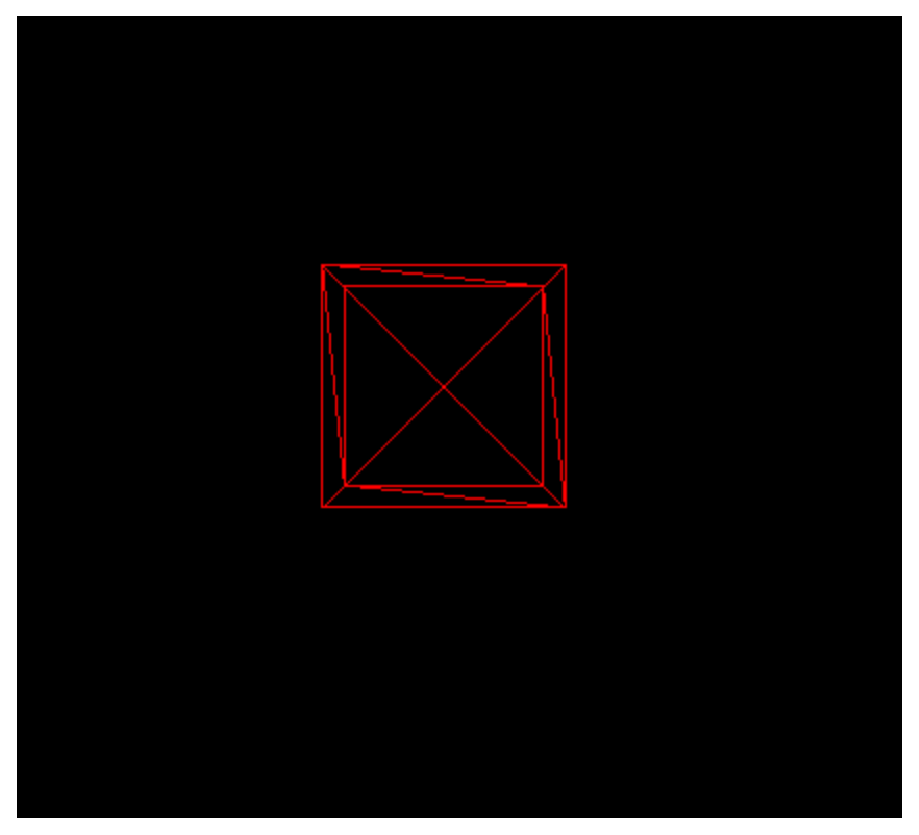
\includegraphics[scale=0.5]{figure/threeexample.eps}
	\caption{Risultato della scena precedentemente creata}\label{fig:threeexample}
\end{figure}

\section{Google Maps API}
Nel primo capitolo di questa tesi ho descritto i più utilizzati sistemi di visualizzazione e navigazione di mappe geografiche disponibili sul web. In particolare, avevo evidenziato come \textit{Google Maps} fosse, probabilmente, il sistema più conosciuto ed utilizzato nel mondo. Sicuramente ciò è dovuto anche alla larga scala di diffusione di smartphones, siano essi con sistema operativo Android di Google o iOS di Apple. All'inizio dello studio del contesto intorno al quale ruotava il mio progetto di tirocinio, una delle prime fasi è stata comprendere quale libreria o API sarebbe stata la prescelta per l'acquisizione delle mappe. Le alternative proposte erano principalmente due: \textbf{Leaflet.js} e \textbf{Google Maps API}. Per descriverle entrambe è necessario sottolineare che la prima è una libreria javascript basata sulle mappe di \textit{OpenStreetMap}, mentre la seconda come si può evincere dal nome è la libreria di riferimento per gli sviluppatori che intendano utilizzare le mappe di Google. La decisione finale, ha portato all'utilizzo delle primitive offerte da Google. 

Le API di Google Maps, sono delle librerie scritte in javascript arrivate alla terza versione, che permettono di interagire, adattare o aggiungere informazioni alla mappa stessa da visualizzare su di un qualsiasi sito web. Per utilizzare le API all'interno di un progetto, è necessario iscriversi gratuitamente alla portale che Google ha destinato agli sviluppatori\footnote{developers.google.com}. Una volta registratosi, lo sviluppatore che intende utilizzare un determinato servizio deve far richiesta di una \textit{API Key}, che permetterà a Google di tracciare l'utilizzo delle mappe all'interno di un sito web. Questo è legato al fatto che l'utilizzo è sì gratuito, ma fino ad un certo limite di richieste giornaliere, il piano standard consente la richiesta di 25000 mappe giornaliere per un massimo di 90 giorni consecutivi, in eccesso Google chiede il pagamento di 0,50 dollari ogni altre 1000 richieste. Queste librerie sono disponibili per differenti target. Accedendo alla documentazione\cite{goo:maps}, è possibile vedere che la stessa è divisa in quattro principali sezioni: \textbf{Android}, \textbf{iOS}, \textbf{Web} e \textbf{Web Services}. Le prime due sezioni riguardano lo sviluppo di applicazioni per i dispositivi mobili con rispettivamente il sistema della stessa casa di Mountain View e quello di Apple. Le altre due sezioni invece riguardano le altrettante componenti di un sito web, perchè con \textit{Web} si intendono tutte quelle operazioni atte a mostrare la mappa sul client, ovvero il nostro browser web. Con \textit{Web Services} si vuole intendere tutte le restanti operazioni di elaborazione che ci servono nel nostro backend, come riportato sulla documentazione ufficiale potremo dunque: accedere al \textit{Geocodice}, ovvero tutte quelle operazioni di conversione tra coordinate geografiche e indirizzi veri e propri; utilizzare servizi di \textit{Geolocalizzazione}, i servizi di posizionamento fruibili da un cellulare con sensore GPS o tramite i nodi WiFi; l'altitudine di ogni posizione della terra, Google ha infatti all'interno dei propri database le informazioni di altitudine di ogni zona della terra (informazioni visibili anche sul portale maps nella vista satellitare prospettica). Quelle elencate sono solo alcune delle principali funzioni disponibili per i Web Services.

Per importare le API all'interno del nostro progetto sarà sufficiente aggiungere un tag "script" all'interno del file HTML, come nell'esempio che segue.
\begin{lstlisting}
<script src="https://maps.googleapis.com/maps/api/js?key=API_KEY
	&callback=initMap"async defer></script>
\end{lstlisting}
Nell'esempio richiamiamo una funzione, initMap, che serve ad inizializzare la nostra mappa. La funzione, prima citata può essere scritta nel modo seguente:
\begin{lstlisting}
var map;
function initMap() {
  map = new google.maps.Map(document.getElementById('map'), {
    center: {lat: -34.397, lng: 150.644},
    zoom: 8
  });
}
\end{lstlisting}
Nella funzione viene creata una mappa con centro nel punto di latitudine -34.397 e longitudine 150.644 e zoom pari a 8. La definizione dello zoom la vedremo più avanti, in quanto è stato uno degli argomenti di studio iniziali del mio progetto.

La natura del mio progetto non era però probabilmente adatta per l'impiego di una mappa già interattiva come quella offerta da Google all'interno del suo servizio. Dovendo lavorare su di un piano tridimensionale, disegnato con Three.js, non era completamente funzionale far interagire tra loro due sistemi già interattivi. Per questo motivo ho deciso di utilizzare un altro servizio più semplificato messo a disposizione da Google. Sto parlando delle Google Static Maps. Le mappe statiche offerte da google sono delle immagini definite in base alla richiesta da noi avanzata. Infatti non c'è bisogno di alcun codice definito o particolare per richiedere la mappa. Questa è disponibile grazie ad un url di richiesta, una vera e propria query, a cui vengono concatenati i parametri necessari: centro, che può essere definito con coordinate polari o con un indirizzo testuale; la grandezza dell'immagine, definita come \textit{LARGHEZZA}x\textit{ALTEZZA} e inifine il livello di zoom desiderato. All'url è possibile attaccare anche altri parametri nel caso volessimo modificare lo stile della mappa, i colori, se volessimo aggiungere dei fermaposto sulla nostra tile o se volessimo disegnare un tracciato su di essa. Un esempi di url di richiesta può essere questo: 
\begin{lstlisting}
https://maps.googleapis.com/maps/api/staticmap?center=Roma,IT
	&zoom=11&size=640x640
\end{lstlisting}
In questo url troveremo una mappa centrata in Roma di zoom 11 e grandezza 640x640 pixels, che è la grandezza massima che Google consente di utilizzare nelle API gratuite. Il risultato dell'url può essere visto nella figura \ref{fig:staticmap}
\begin{figure}[ht]
	\centering
		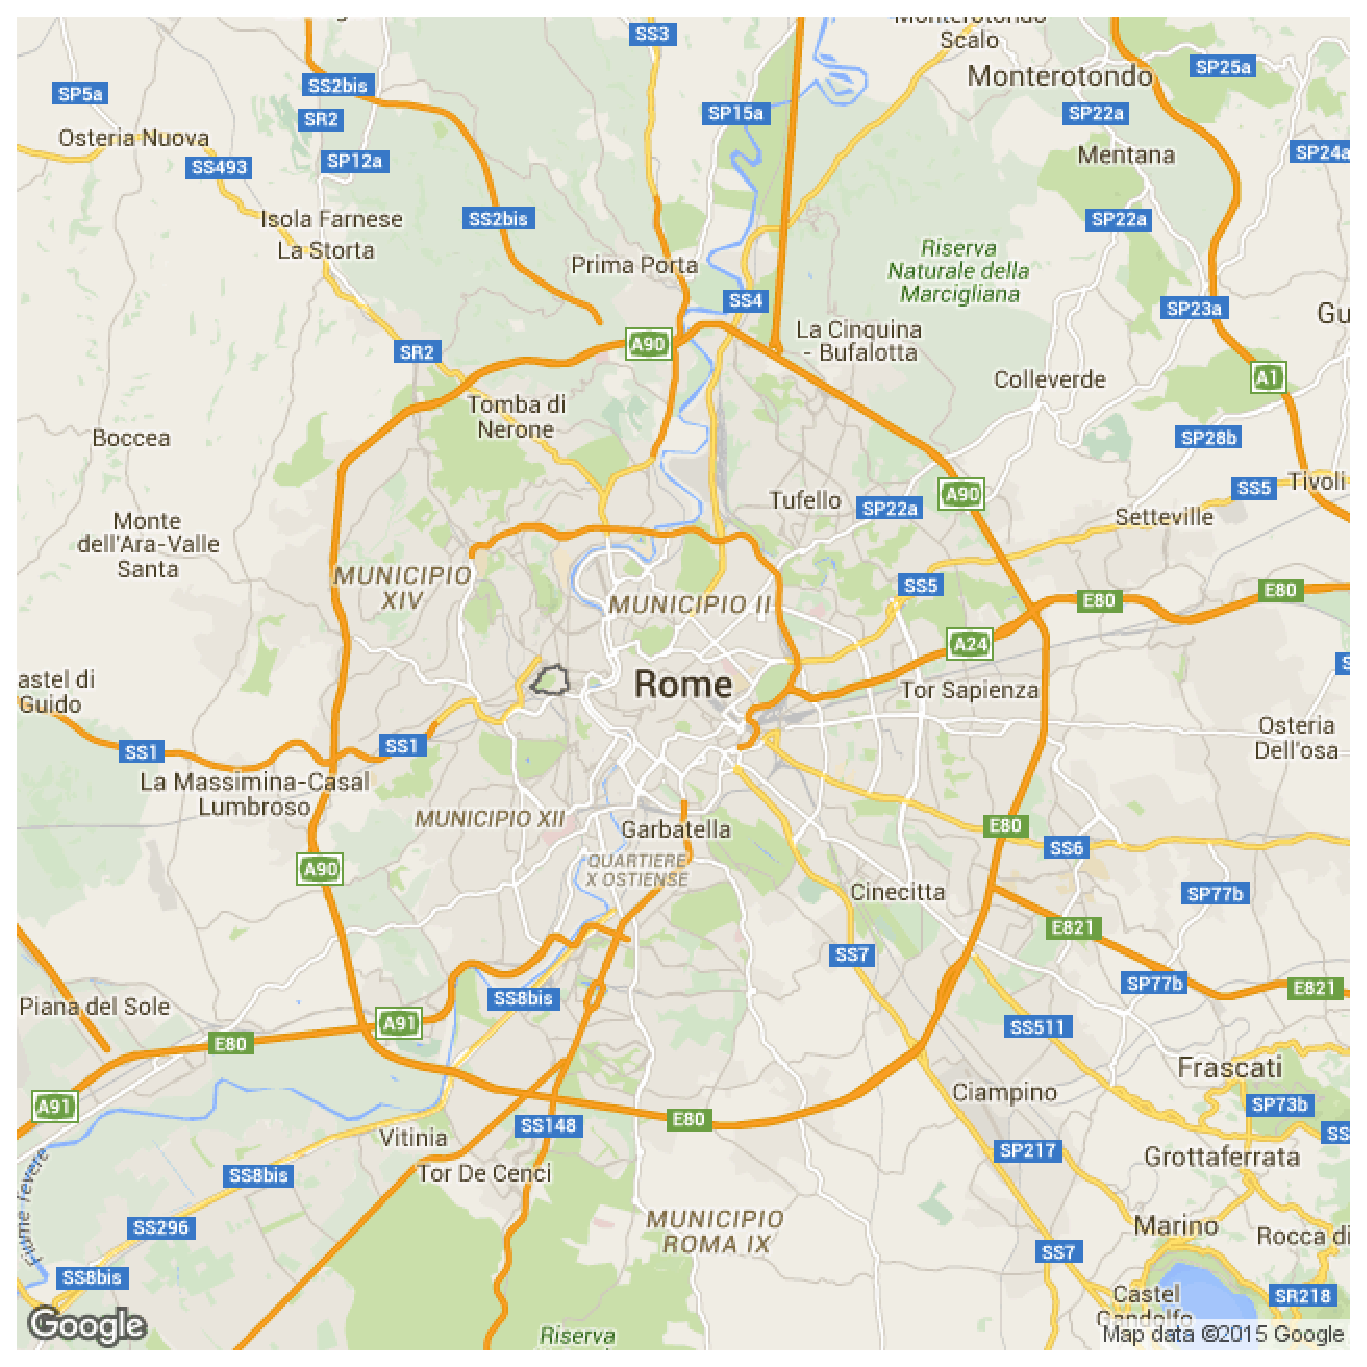
\includegraphics[width=\textwidth]{figure/staticmap.eps}
		\caption{Esempio di mappa statica di Roma}\label{fig:staticmap}
\end{figure}